\chapter{Experimental Results}
\label{sec:ExperimentalResults}

In order to evaluate the efficiency of the designed packages and also the Apriltag's detection algorithm, a series of experiments were conducted both in simulation and with the real system.

\section{Experiments Conducted in Simulation}
\label{sec:simulatedExperiments}

In order to evaluate the simulated system, the ability of the MAV to track and follow the Apriltag under various conditions was tested. As mentioned in \ref{sec: apriltagFireflySimulation} there are two offsets added in the robot's reference frame, these target to the security of the user, so as to avoid collision, and also to provide the MAV with a better field of view, thus improve the Apriltag detection rate.   

In the first experiment, we prove that the MAV always leaves an almost constant distance between itself and the detected marker. First the user presents the Apriltag that commands the MAV to hover. Then the marker that commands it to follow, after that the program automatically rotates this marker inside the simulation with a constant predefined turning rate. This is accomplished by changing the marker's yaw, while leaving the position unchanged. The tested rates are $0.5^{\circ}$, $2^{\circ}$ and $5^{\circ}$ per frame and since in simulation the USB camera records with 30 fps, the rates are of $15^{\circ}/sec$, $60^{\circ}/sec$ and $150^{\circ}/sec$ respectively. In figure \ref{pics:xyRotation}, only the x and y coordinates are presented. It can be seen that the MAV performs a circle while it follows the tag, thus it leaves a constant distance between itself and the marker. The lines that start from point (0,0) represent the Firefly's trajectory to its initial position relative to the tag. The spikes that appear in the $60^{\circ}/sec$ and $150^{\circ}/sec$ trajectories exist because by the time the MAV reached its initial position the tag had already rotated, thus the robot had to move greater distance. The fastest rotation the MAV can follow is about $240^{\circ}/sec$, at greater rotation speeds the MAV is not able to follow the rotation. Conversely to what was expected, the Firefly has more oscillations in the z axis at the lowest turning rate, as can be seen from figure \ref{pics:zRotationCOntroller}. That is normal since the MAV has to stay at the various positions before it receives the next measurable position value. Thus, the MAV has to stop and continue at all times in order to follow the Apriltag. On the other hand, when the tag is rotated faster the MAV always gets a new position command before it needs to stop and wait for a new one.

\begin{figure}
   \centering
   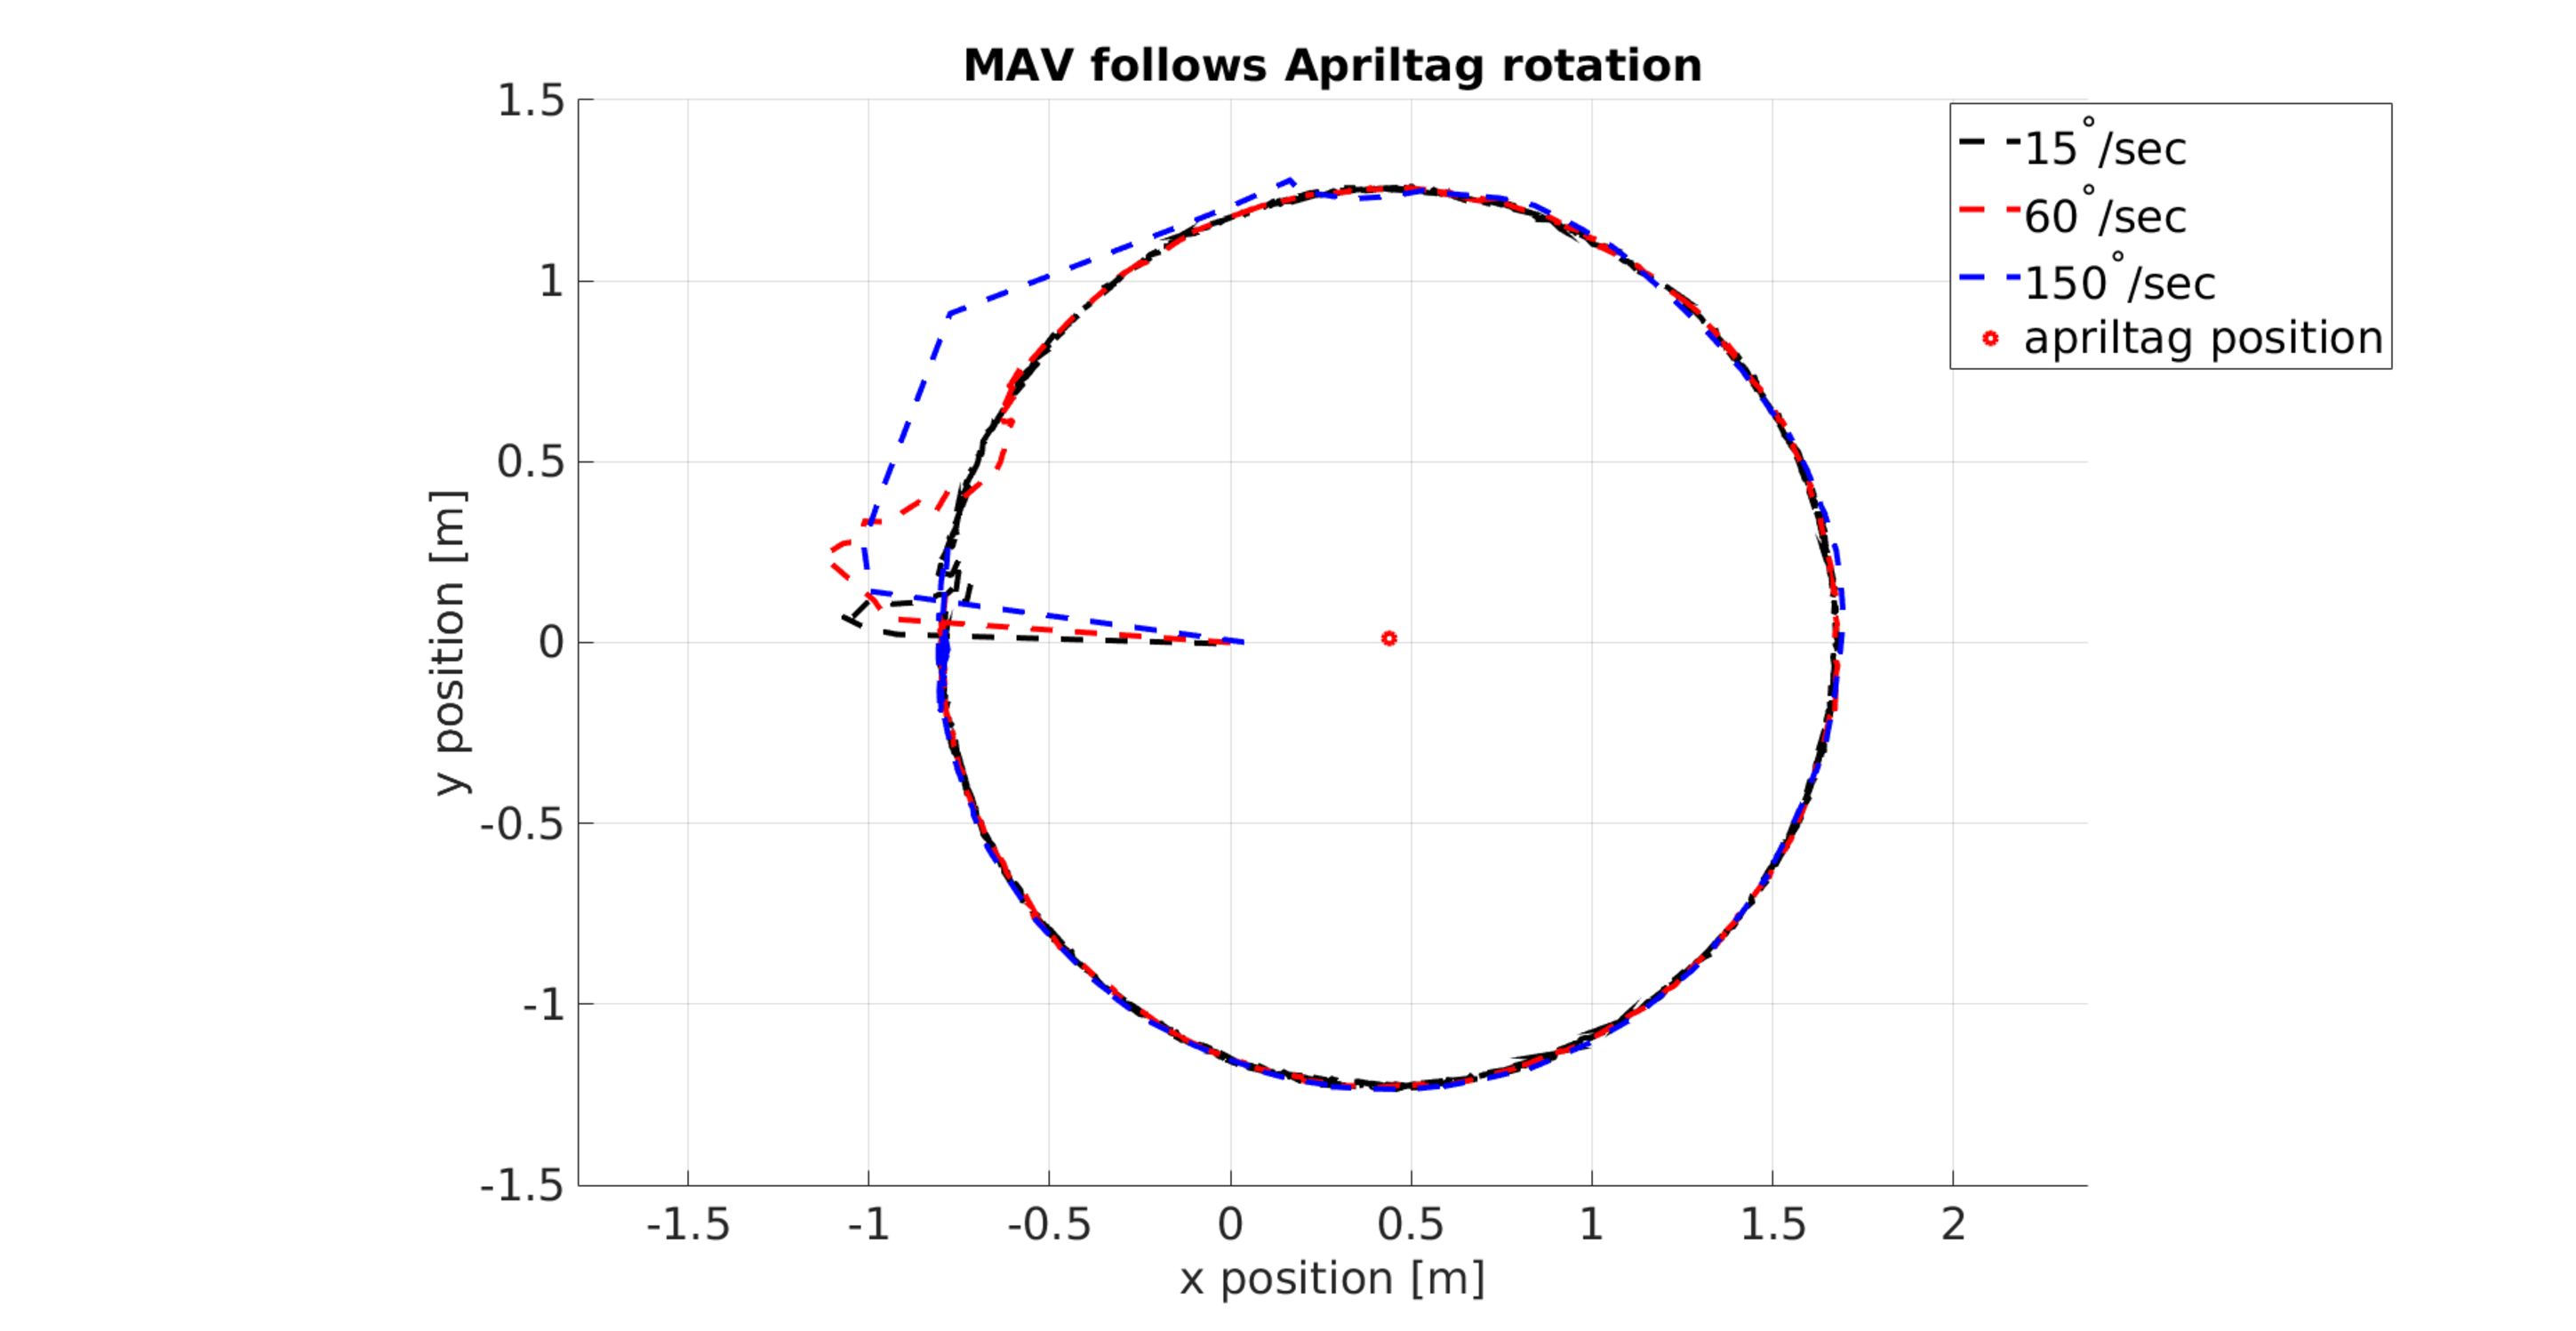
\includegraphics[width=1.00\textwidth]{images/MAV_controller_input_rotation_tracking.pdf}
   \caption{The MAV follows the Apriltag while it rotates around itself}
   \label{pics:xyRotation}
\end{figure}

Furthermore, tests were conducted to test the MAV's ability to follow the tag in different motion configurations. In figure \ref{pics:simLinearMotion} are presented the results of such an experiment. Here the tag is moved, inside the simulated world, following straight line patterns. Again, it can be observed that the Firefly follows the Apriltag under all circumstances. We can observe, that the controller's input data are quite noisy especially at the abrupt orientation changes, thus they have some oscillations of about 0.1m, but the MAV acts like a low pass filter and these high frequency oscillations are not performed by the MAV. During the experiments, it was observed that when the marker was moved at distances further than 2m away from the camera, then the orientation detection became unreliable and changed randomly. Although the algorithm could still measure distance accurately, it had some significant problems reading the correct orientation data from the Apriltag. That misdetection led to very abrupt random motions, since the coordinates sent to the controller use the detected pose of the marker in the transformation from the reference frame to the world frame. 

\begin{figure}
   \centering
   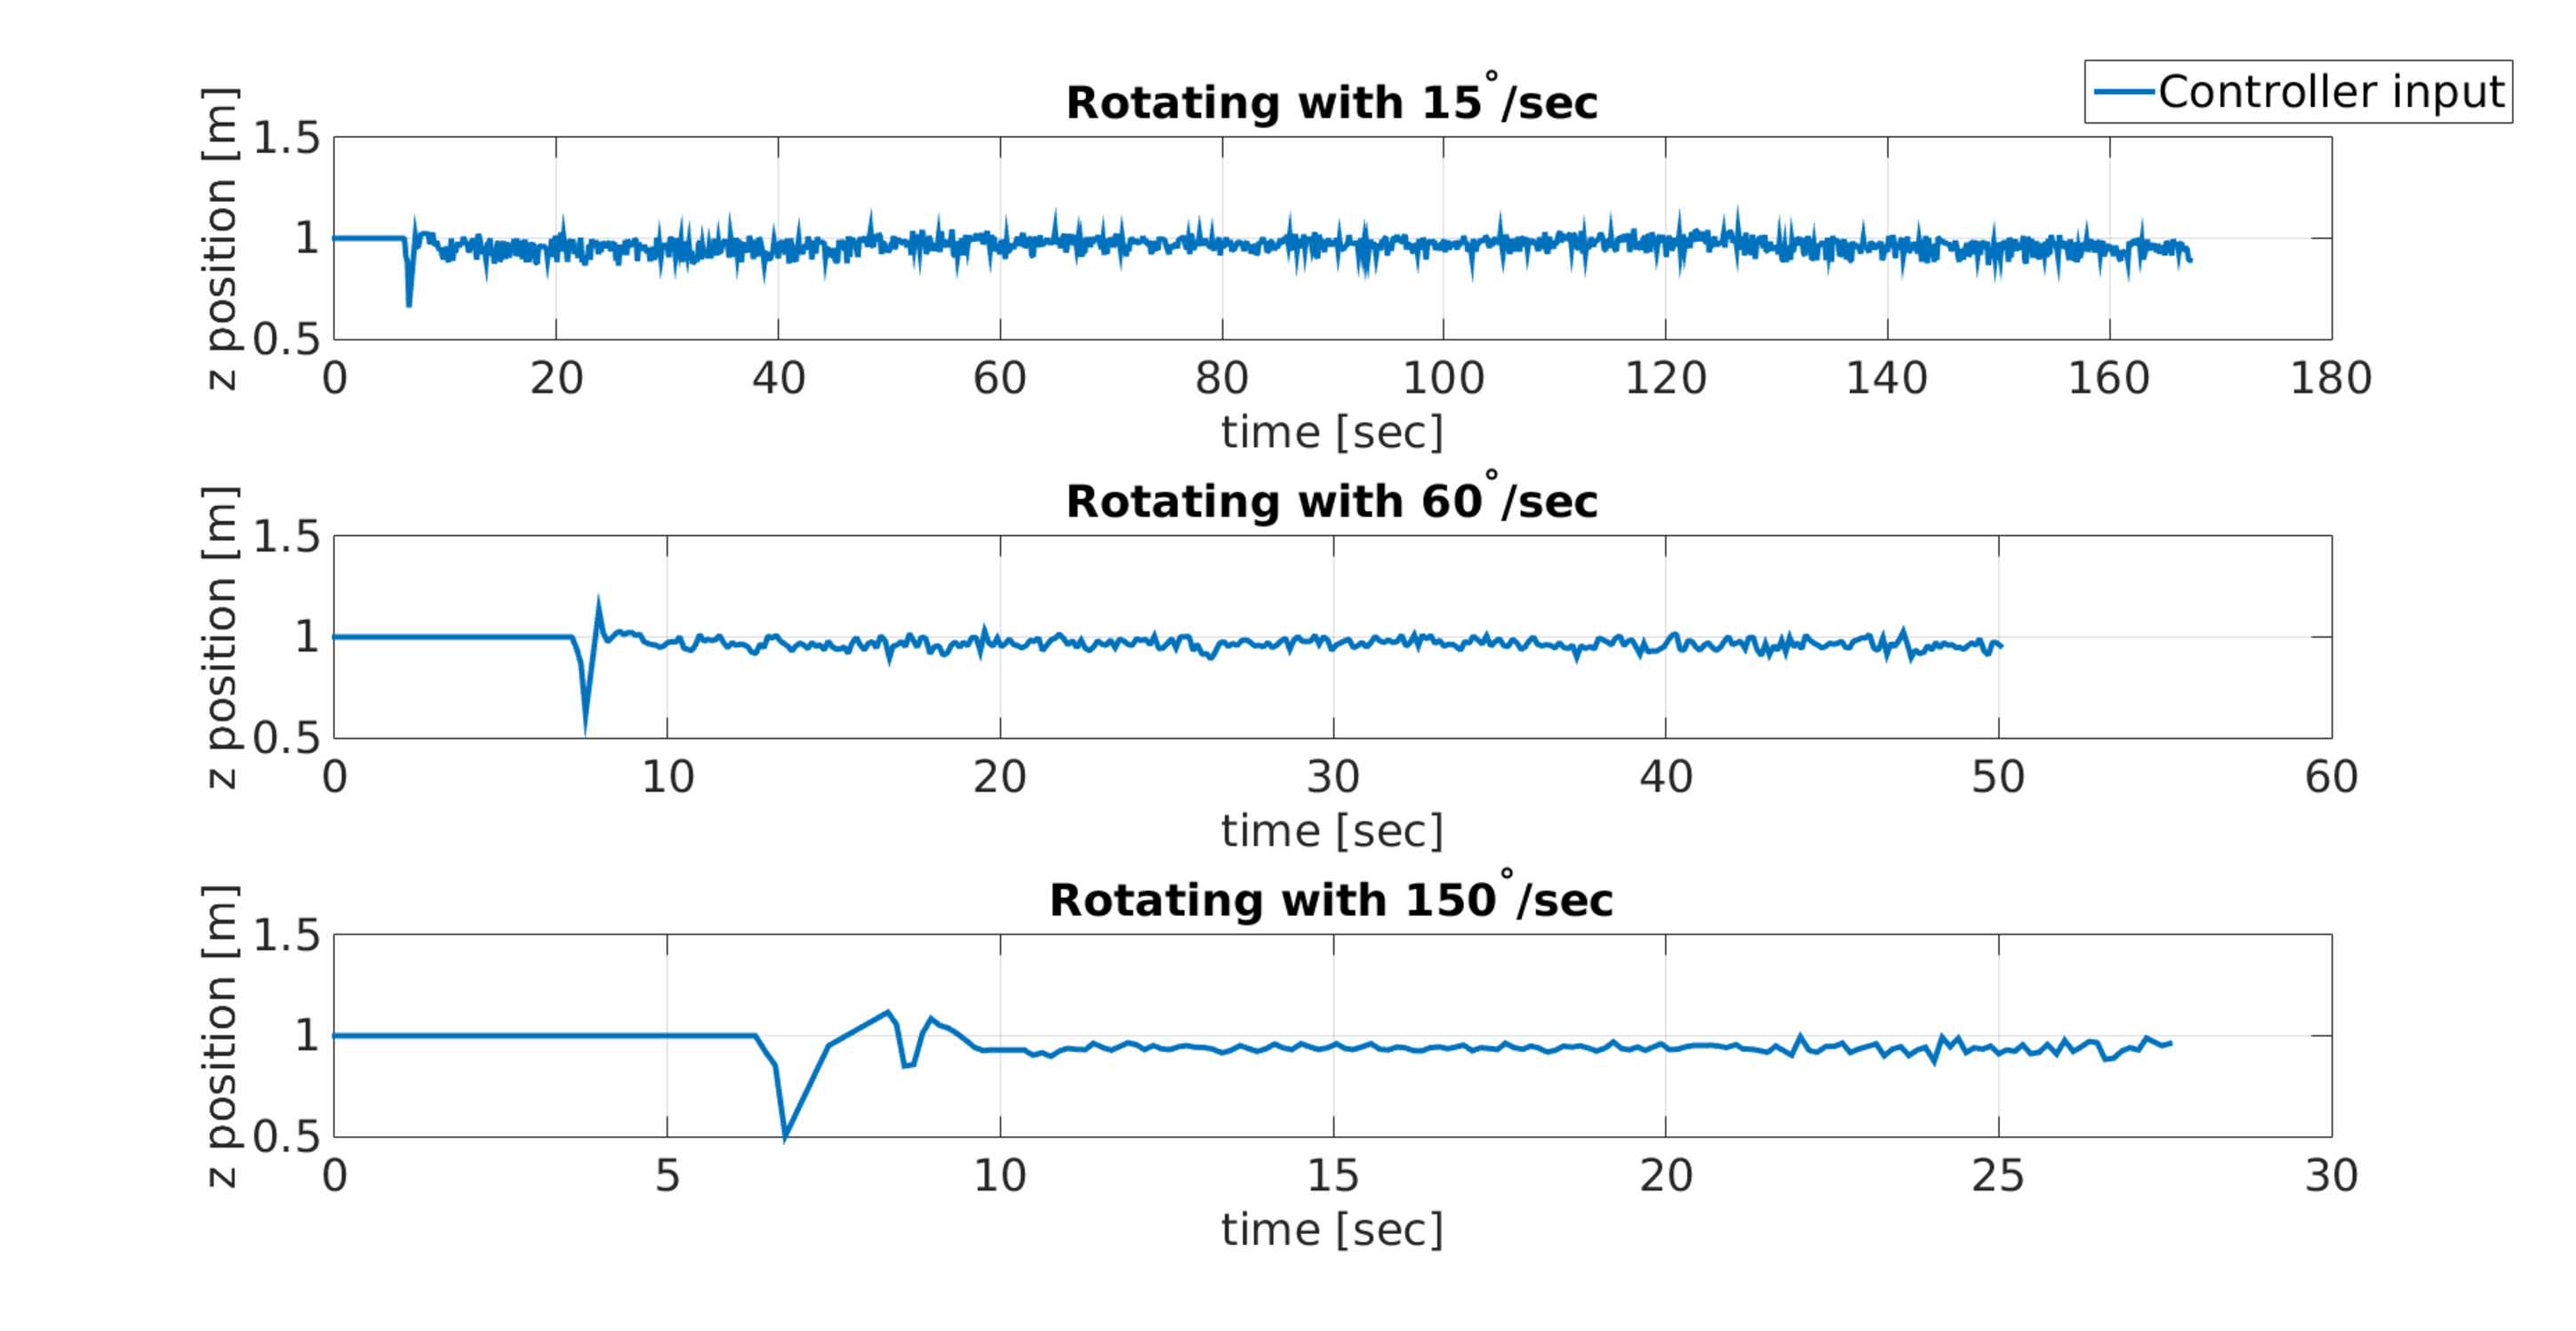
\includegraphics[width=0.98\textwidth]{images/sim_z_axis_during_rotation.pdf}
   \caption{The controller input at z position versus time during the three rotation experiments}
   \label{pics:zRotationCOntroller}
\end{figure}

\begin{figure}
	\centering
	 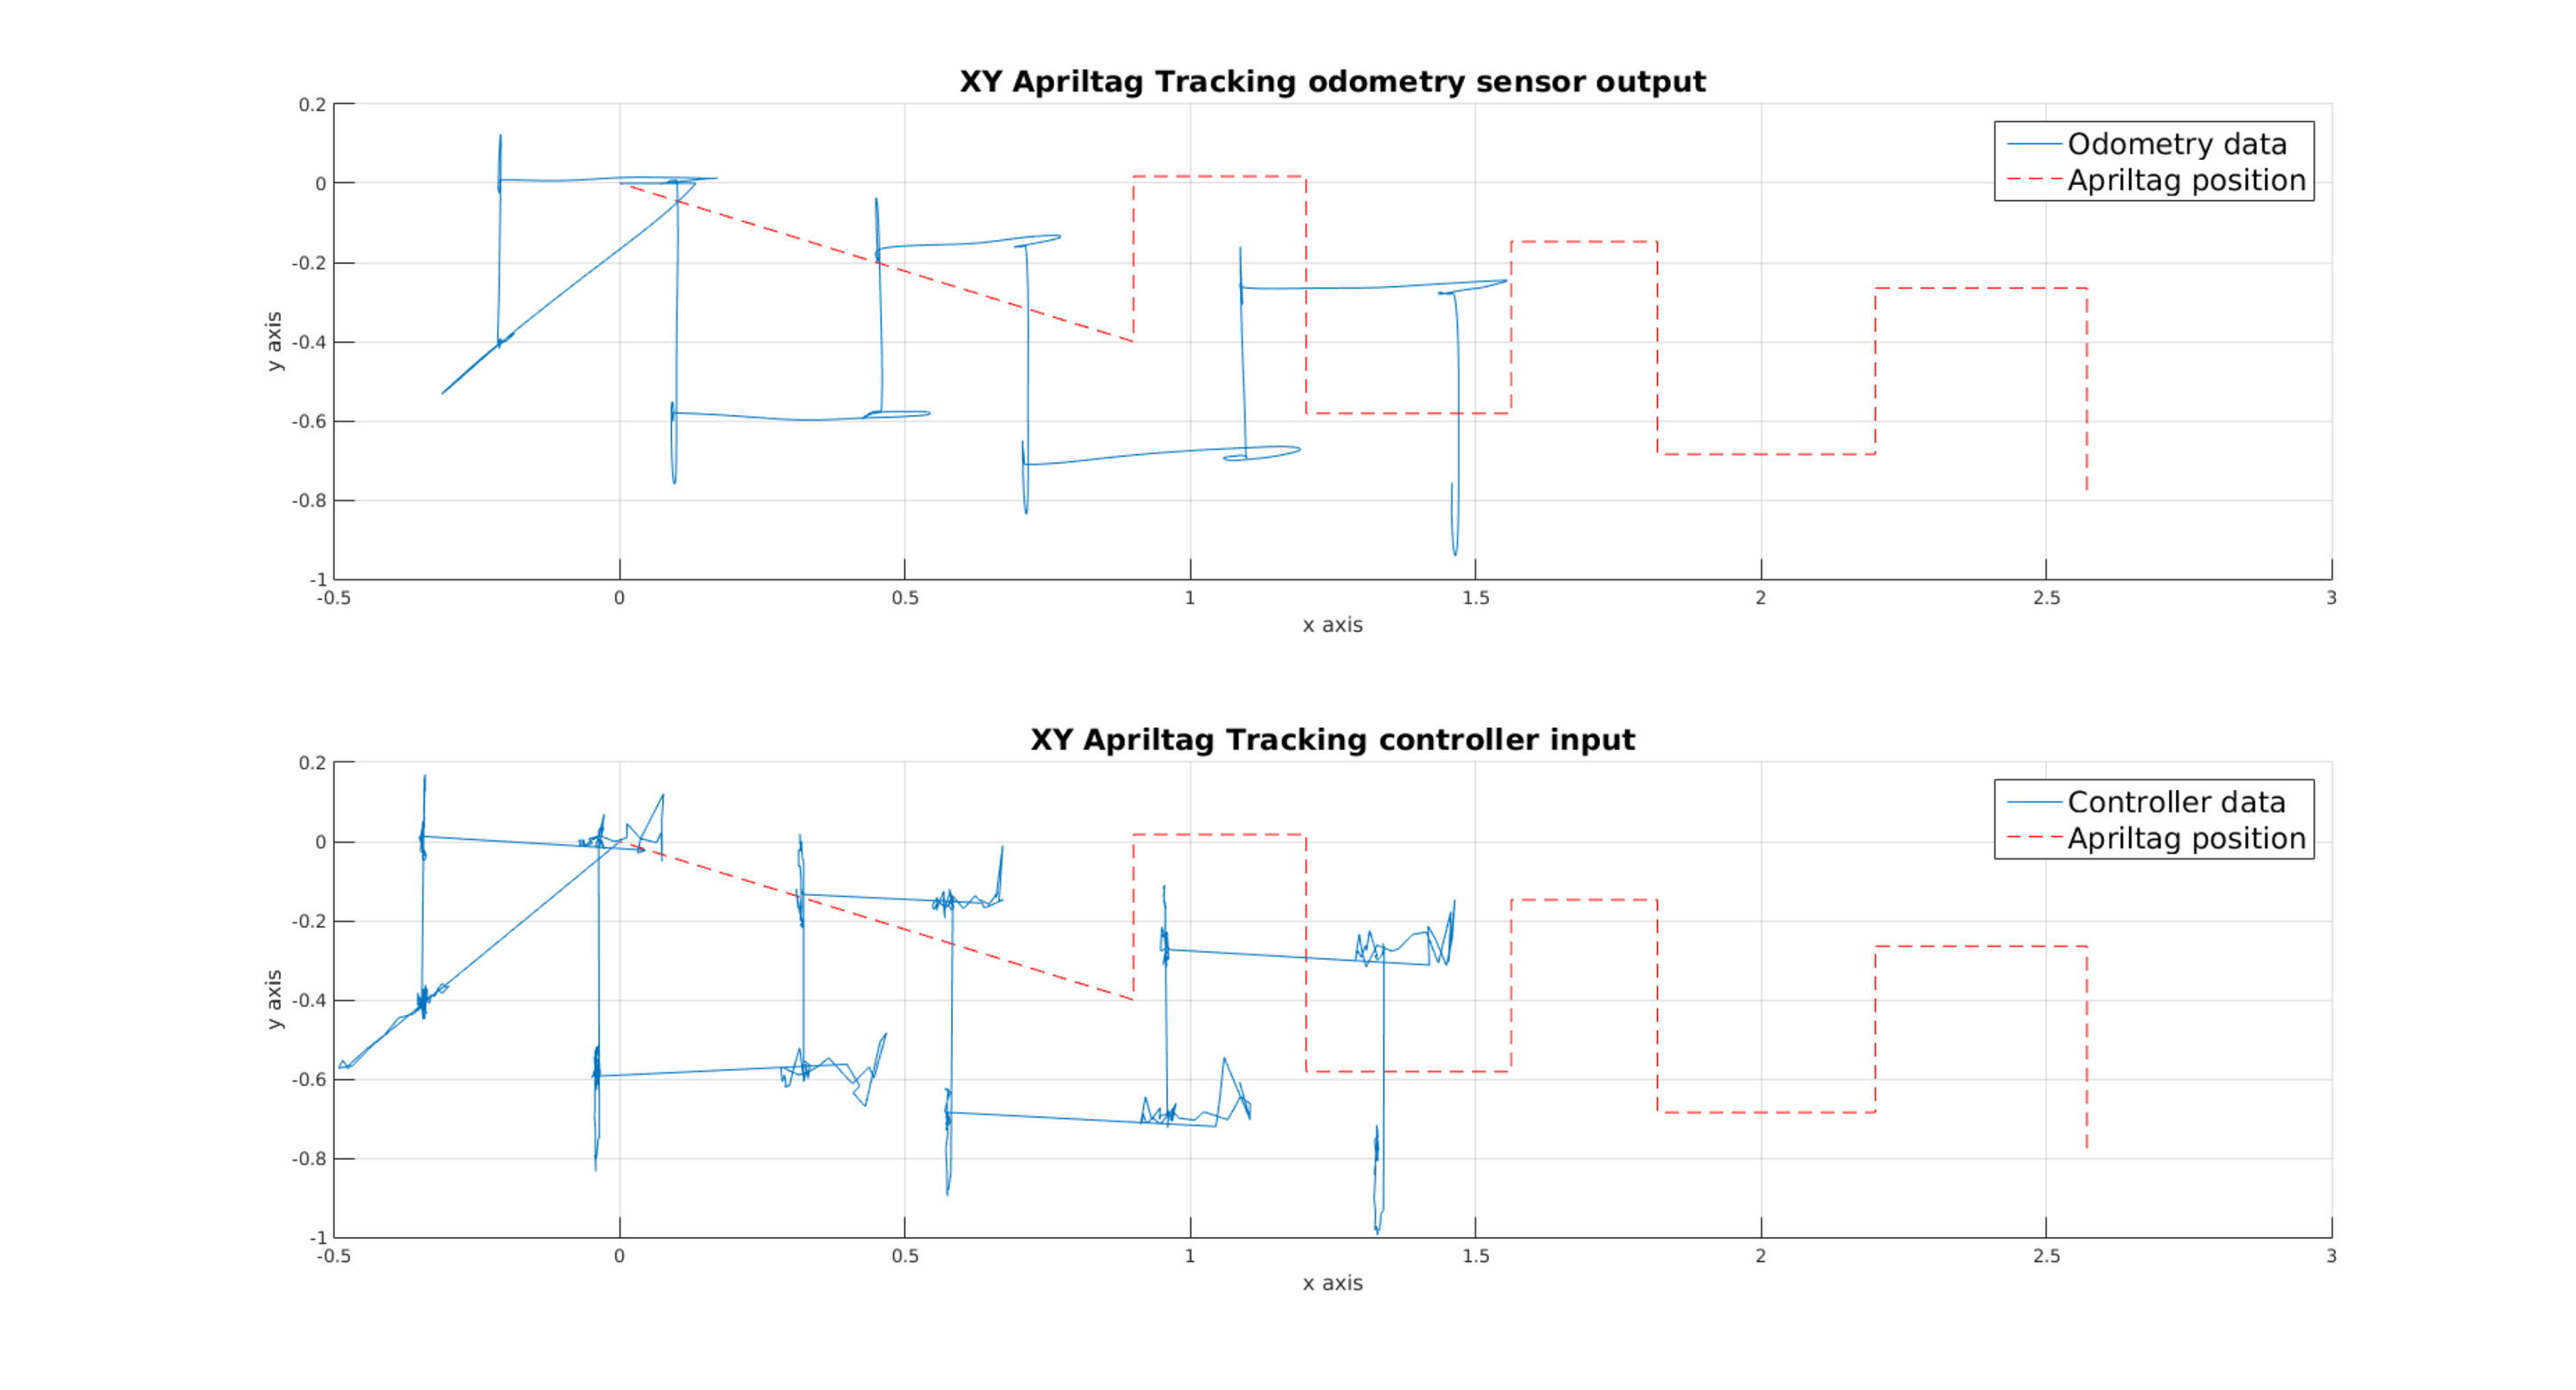
\includegraphics[width=1.00\textwidth]{images/sim_linear_motion.pdf}
	 \caption{The MAV follows the Apriltag in the linear pattern}
	 \label{pics:simLinearMotion}
\end{figure}

 
\section{Experiments Conducted in the Real System}
\label{sec:realExperiments}

In order to validate our system, experiments with a real MAV were conducted. The name of the drone used is "AUK". First of all, it should be mentioned that in order to avoid any dangerous situations, due to the misdetected orientation data, as mentioned in section \ref{sec:simulatedExperiments}, the orientation read from the Apriltag detection algorithm was substituted with a fixed rotation. Thus, the MAV could only follow the marker in straight lines since it did not track the Apriltag's yaw. Furthermore, during the experiments we experienced some difficulties with the onboard odometry system (ROVIO\protect\footnotemark), thus the VICON system was used to provide odometry data.

\footnotetext{https://github.com/ethz-asl/rovio}

Four experiments were performed, in the first three the ability of the MAV to follow a "normally" moving target was tested, while in the fourth experiment the marker motions became faster and more abrupt. It should be mentioned, that during the first experiment we faced some difficulties due to problems with the MAV's trim. The overall Apriltags' detection rates based on the experimental results, are presented in table \ref{table:detctionRates}. In order to compute the detection rate, the number of frames during the manual phases (landing and take off) were excluded from the total number of frames. It can be seen that the algorithm, regardless the motion of the Apriltag achieved at least 90\% detection at all cases. It should be mentioned, that due to the VICON system in the room the lighting conditions were not stable, since the camera sensor could detect the infrared flickering caused by its cameras and also, the onboard camera sensor had only a resolution of 480 x 752 pixels.

\begin{table}
\begin{center}
    \begin{tabular}{ | l | l |}
    \hline
    Experiment & Detection Rate \\ \hline
    $1^{st}$ Experiment & 90.86\% \\ \hline
    $2^{nd}$ Experiment & 96.73\% \\ \hline
    $3^{rd}$ Experiment & 96.3\% \\ \hline
    $4^{th}$ Experiment & 93.16\% \\ \hline
    \end{tabular}
    \caption{The Algorithms detection rates in the four conducted experiments}
    \label{table:detctionRates}
\end{center}
\end{table}

\begin{figure}
	\centering
	 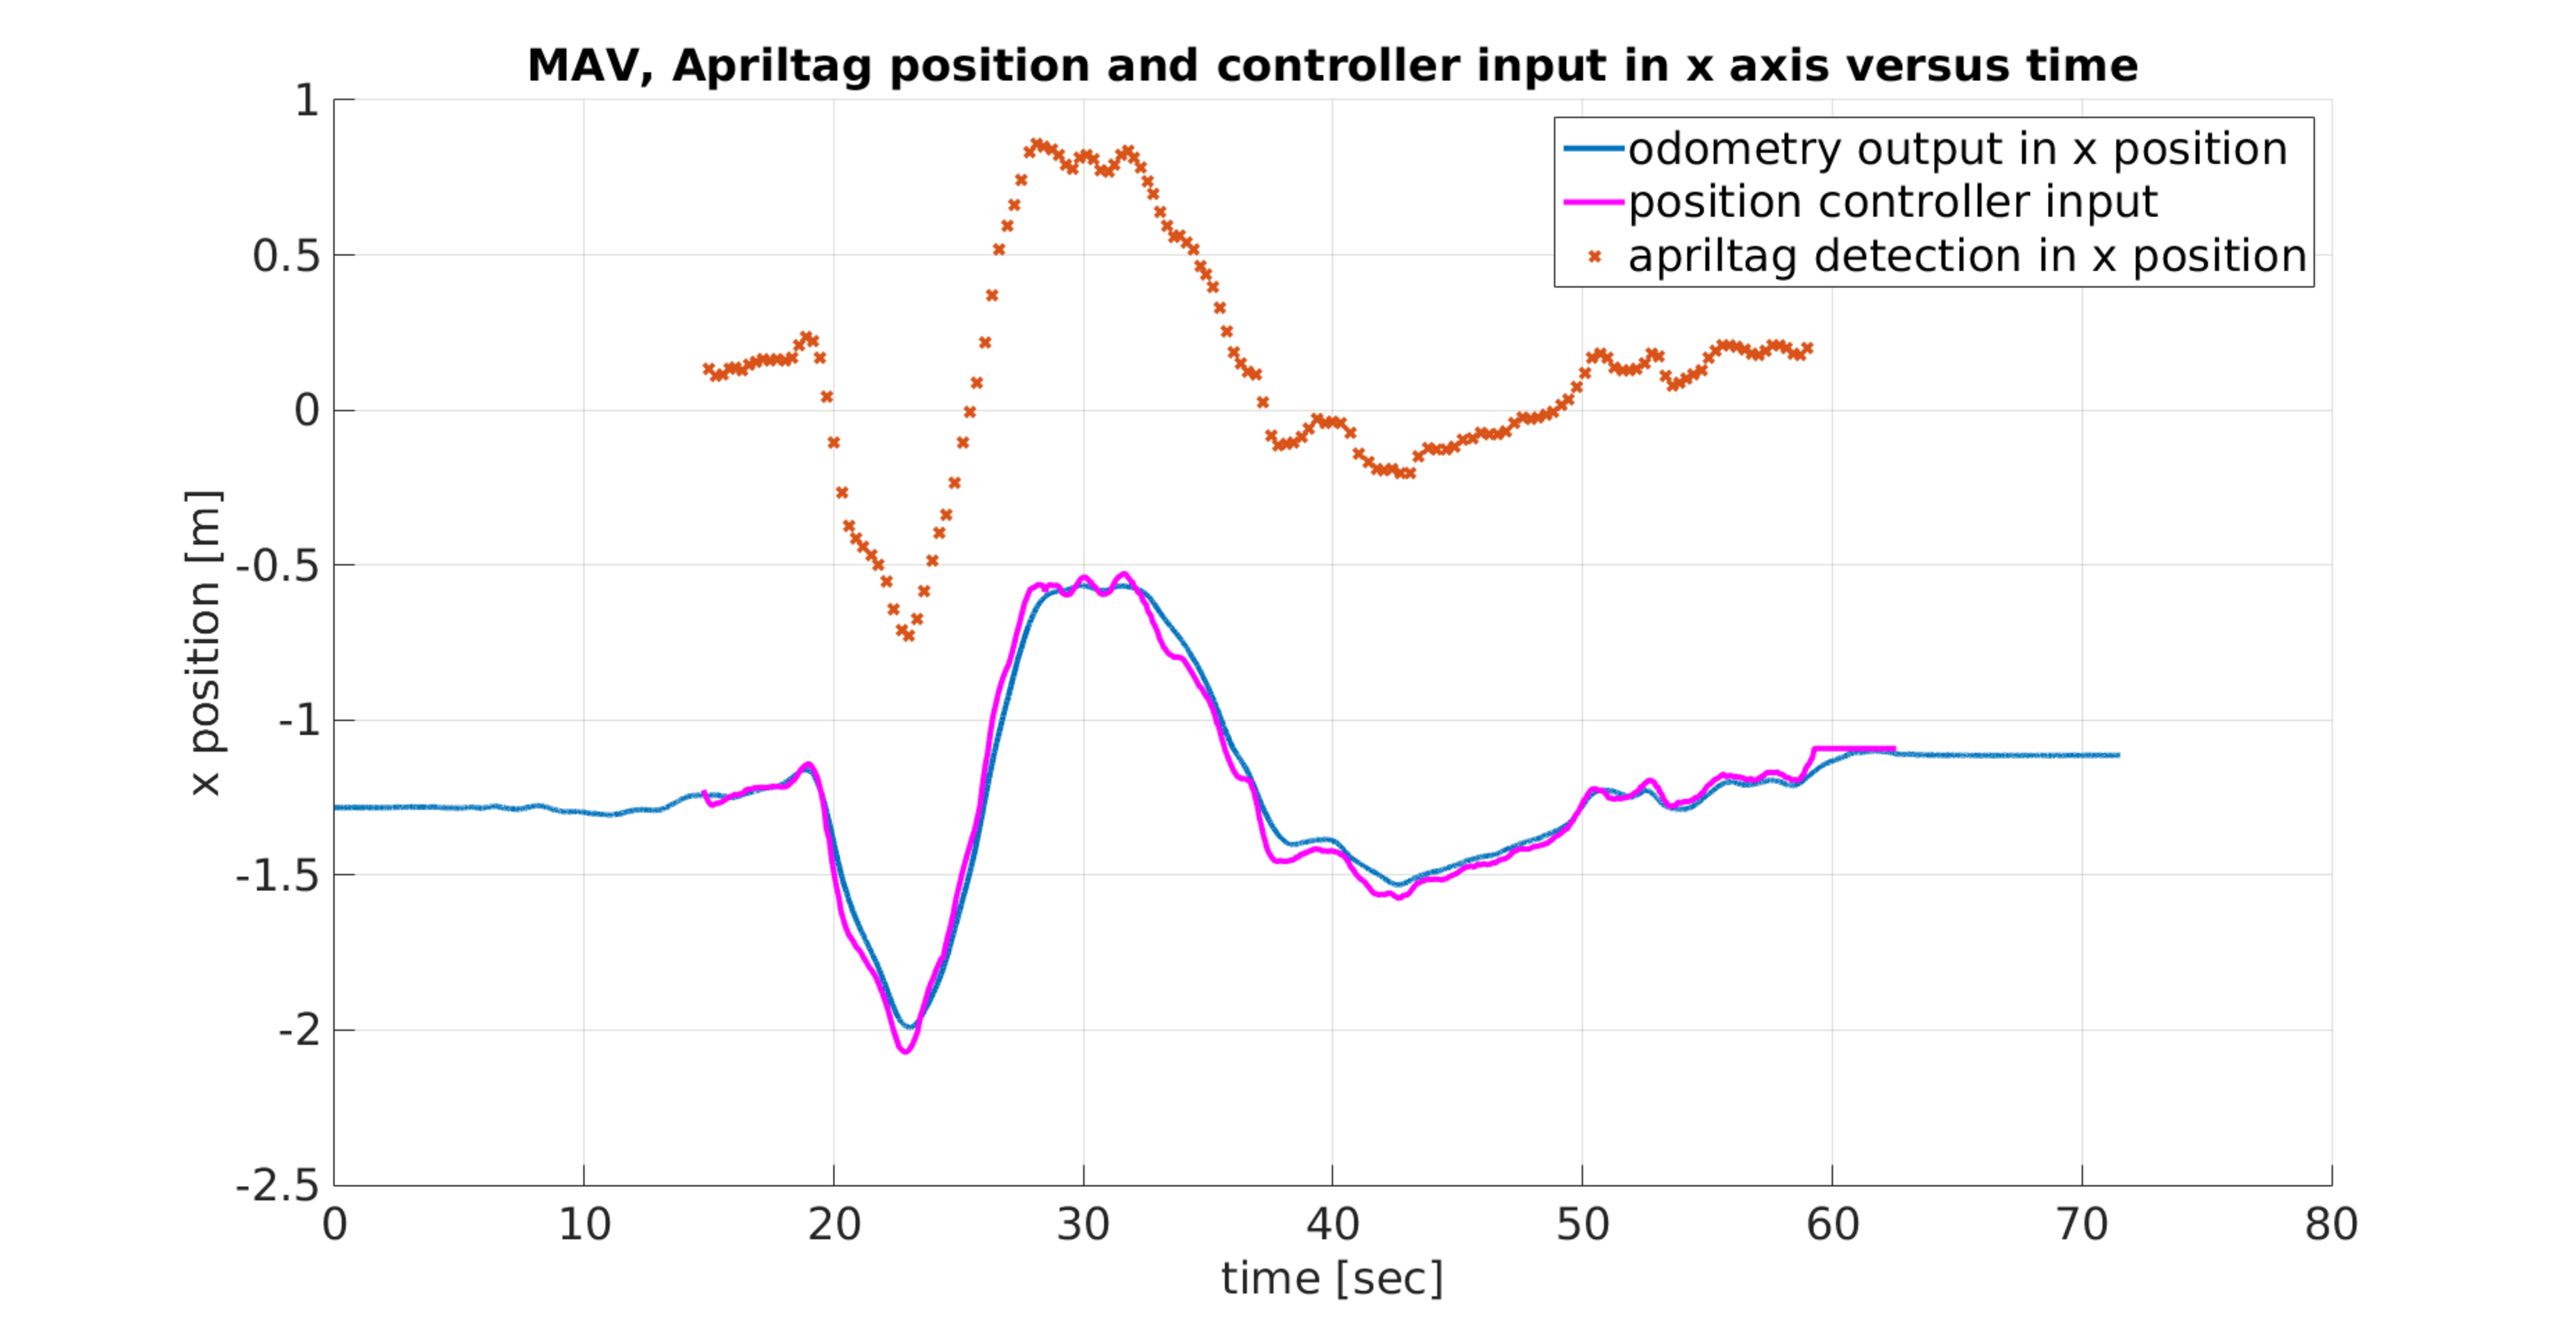
\includegraphics[width=1.00\textwidth]{images/real_MAV_odom_controller_bag3.pdf}
	 \caption{The odometry output against the controller input and the apriltag detection position versus time.}
	 \label{pics:realOdomControlDetection}
\end{figure}

\begin{figure}
	\centering
	 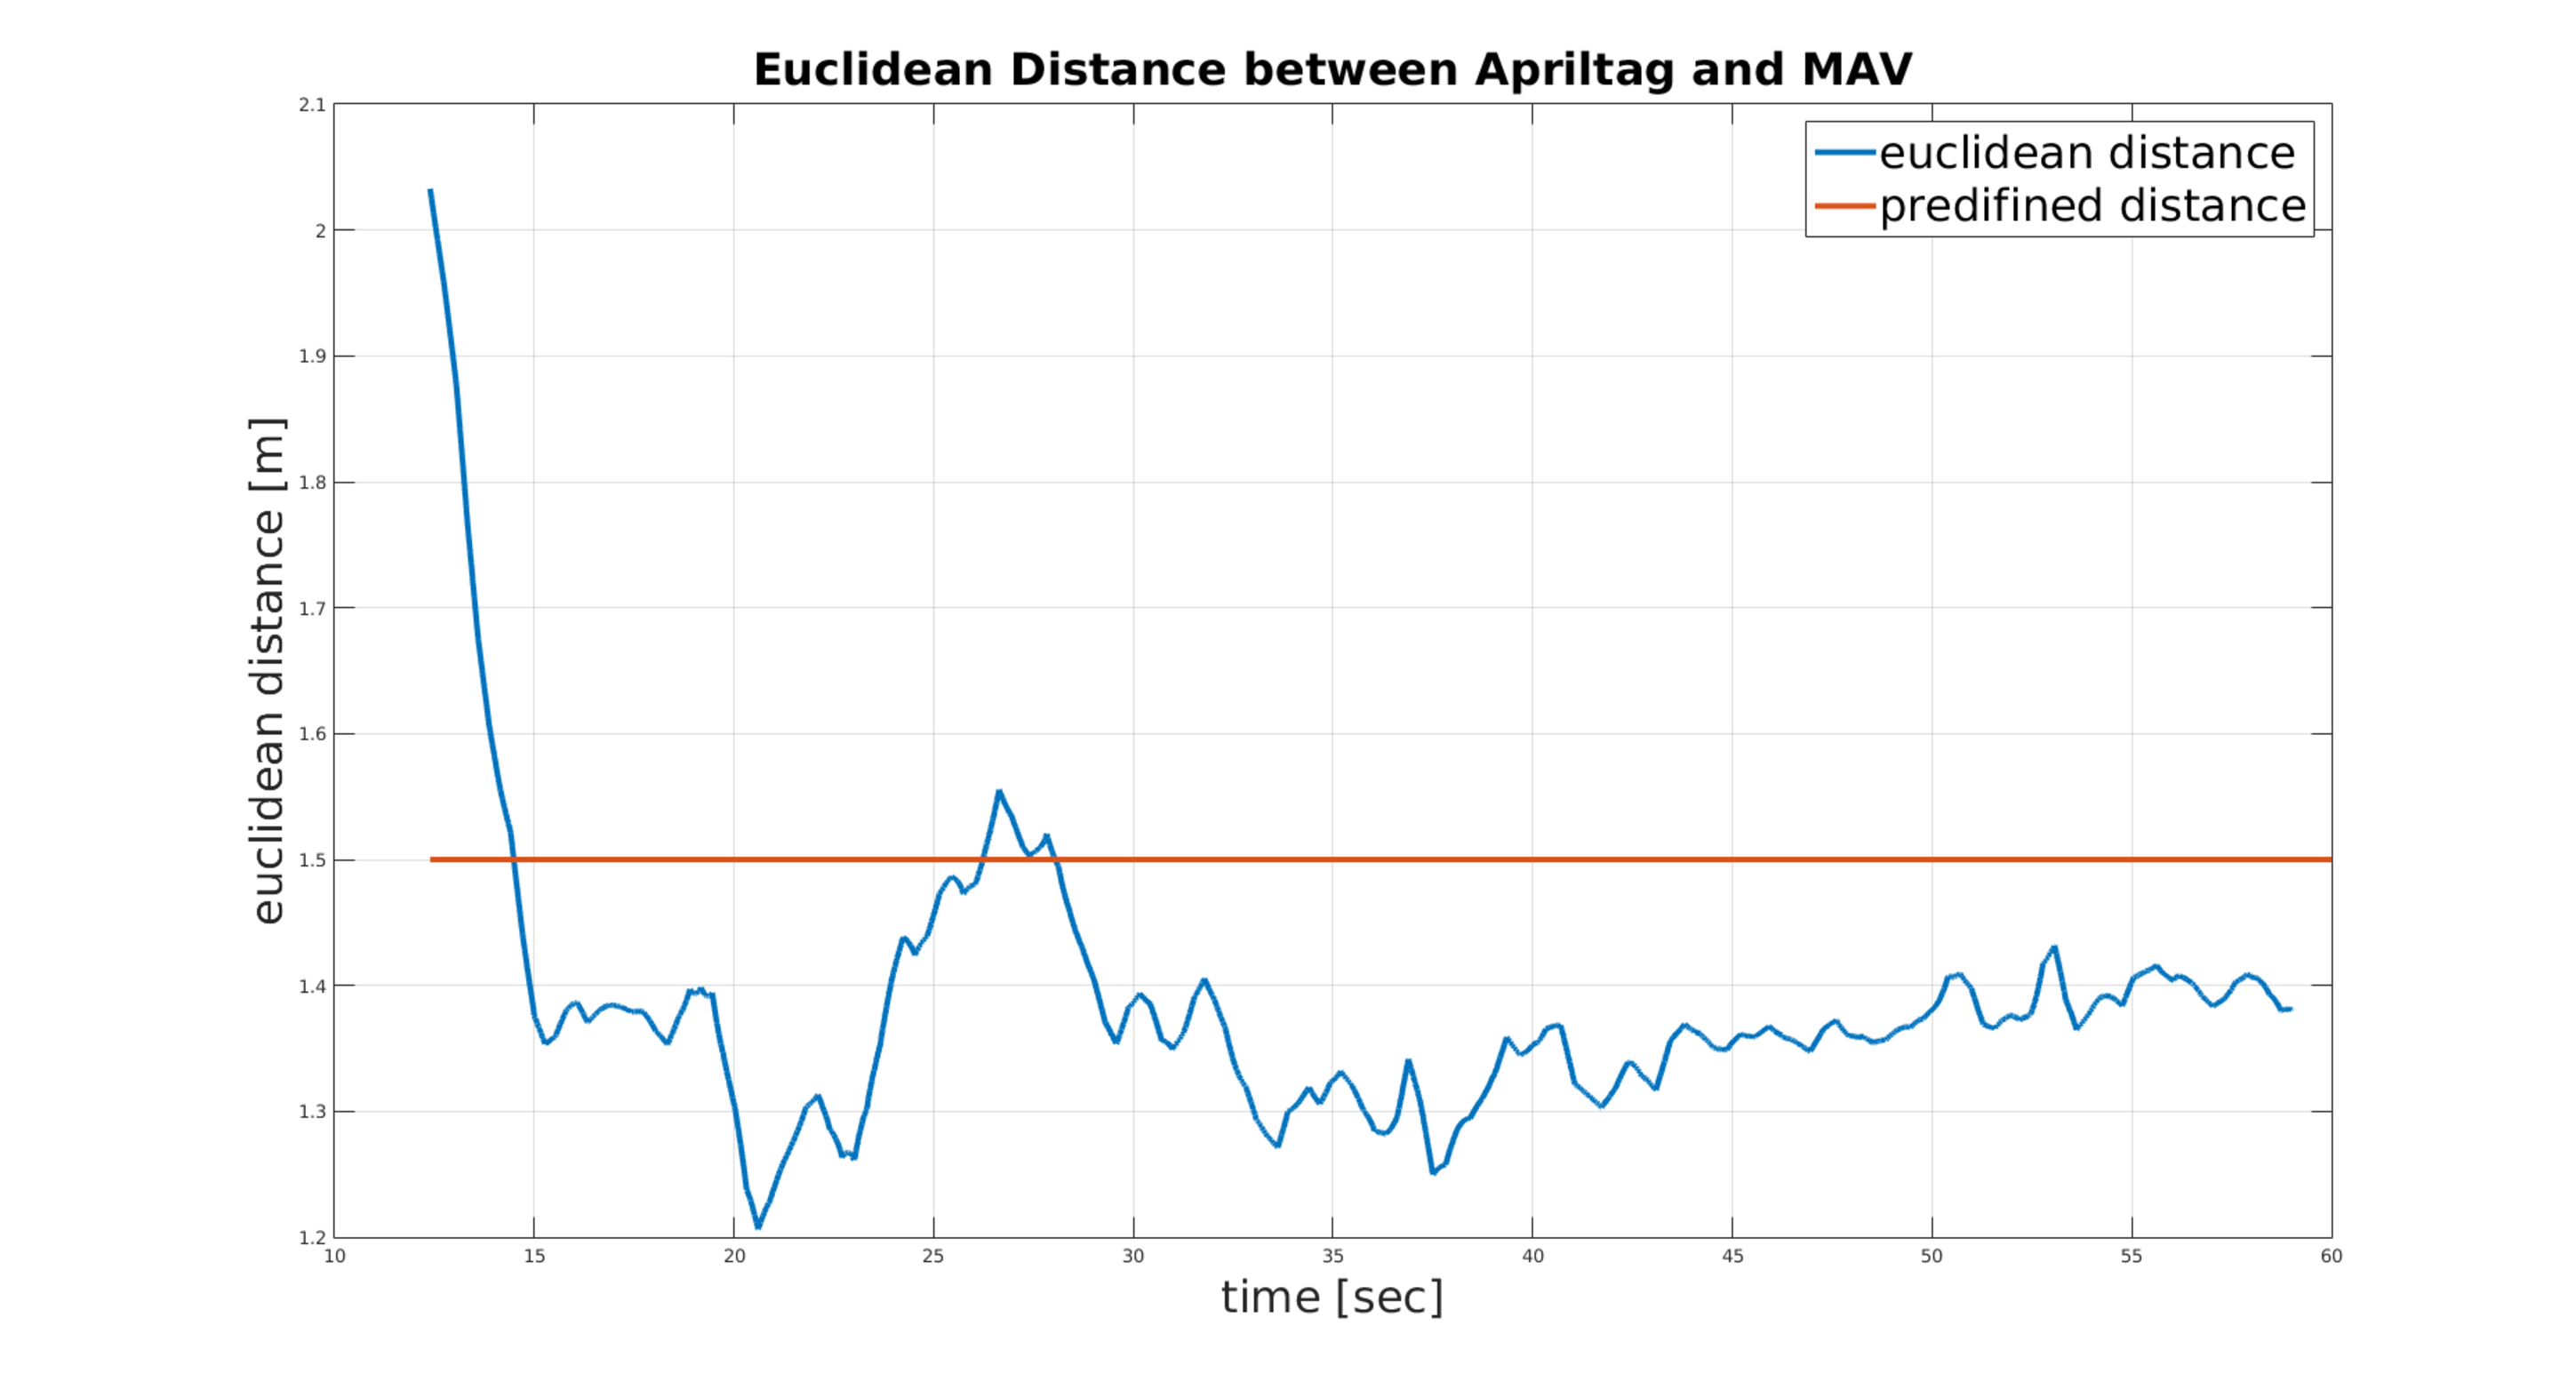
\includegraphics[width=1.00\textwidth]{images/real_euclidean_distance.pdf}
	 \caption{The euclidean distance between the MAV and the Apriltag at x axis}
	 \label{pics:euclideanDistance}
\end{figure}

Since the nature of the experiments is very much alike to each other, only one set of data will be presented. As can be seen from figure \ref{pics:realOdomControlDetection}, the MAV manages to track the marker and follow it under all circumstances. The MAV, acts like a low pass filter on the controller inputs, thus it smoothens the aforementioned as it can be seen from the odometry output. Furthermore, we can observe from figure \ref{pics:euclideanDistance} the euclidean distance between the Auk and the marker with respect to x axis as it proceeds in time. Although the distance between the MAV and the user is, almost at all cases, less than the predefined safety distance, the MAV always leave adequate distance as it can be seen from figure \ref{pics:experimentCapture}. The reason for not always achieving the safety distance, is that the user moves the Apriltag before the MAV has reached that predefined distance, but even in this case, the average error from our desired safety distance is only 11.67 cm.   

\begin{figure}
	\centering
	 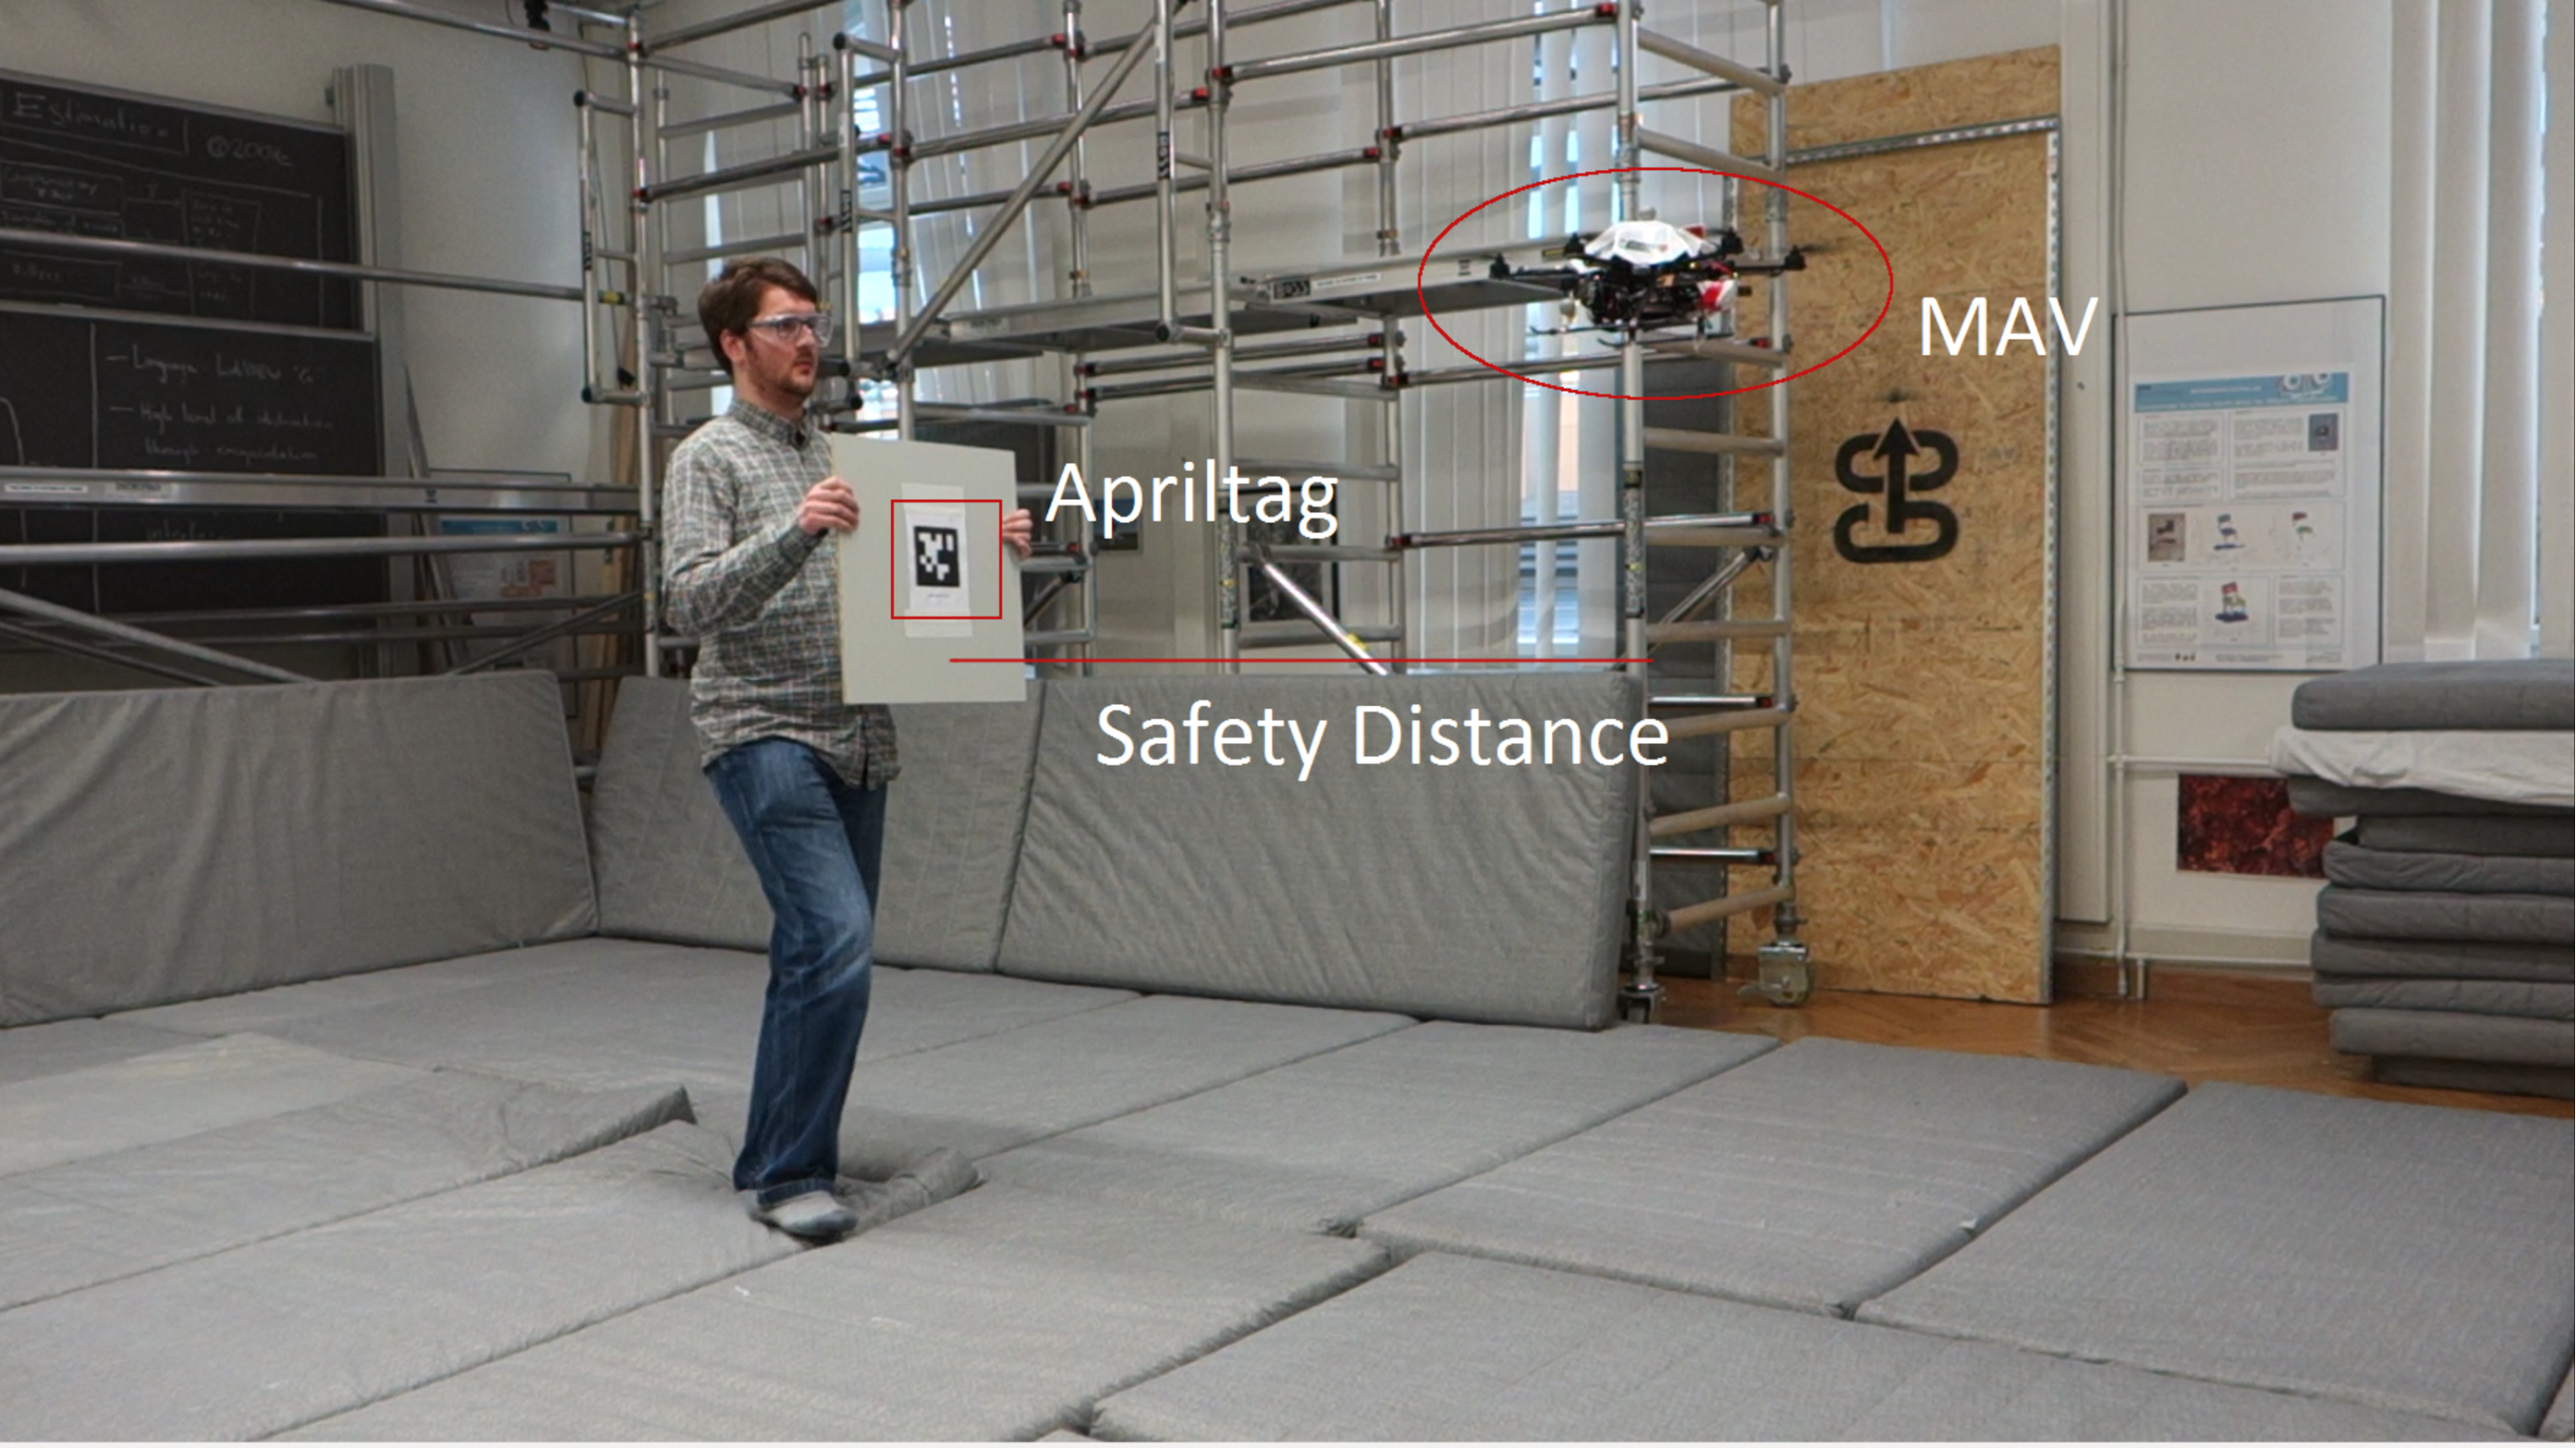
\includegraphics[width=1.00\textwidth]{images/real_experiment_v1.pdf}
	 \caption{The actual experimental setup}
	 \label{pics:experimentCapture}
\end{figure}

During the last experiment, the ability of the algorithm to track faster and more abrupt motions was tested. During this experiment, some discontinuities in the MAV's motion were observed, they were caused by the instantaneous loss of the Apriltag detection, since the user moved the marker fast from one position to another. During the time between the last observed marker position and until a new detected position was created from the detection algorithm, the MAV's controller was receiving as target position the last position where the marker was detected. Thus, this led to short sudden holds in the MAV's trajectory. During the analysis of the data, it was observed that the periods when the MAV could not detect the Apriltag varied between two to nine frames, or 66 to 300 msec. It should be mentioned, that the aforementioned cases refer only in situations where there is a loss of detection and not when the user moved the Apriltag out of the field of view of the MAV's camera. But even in the latter cases, the MAV was able to regain the marker detection since it had already started moving to its direction.   

